
\lhead[\chaptername~\thechapter]{\rightmark}


\rhead[\leftmark]{}


\lfoot[\thepage]{}


\cfoot{}


\rfoot[]{\thepage}


\chapter{Application Mapping on NoCs}


\section{Overview}

NoCs (or SoCs in general) are being developed to improve the computational
acumen at our disposal. We want better performance ( that can be associated
to QoS) for real life applications such as word processors , media
players and high-end graphics. This leads us to our next problem.
How to map the applications, that were previously trivially implemented
as serial, on a many-core. Unfortunately it turns out that all task
allocation problems for NoCs can be modeled as bin-packing problem
( a NP complete problem ) . 

Fortunately , it isn't the end of it. There are efficient algorithms
that give decent allocation results in practice. Further , though
the allocation of tasks on processors can be reduced to bin packing,
we also need to pay attention to minimizing communication.

Thus we are faced with a tradeoff.

Linear clustering , targets close allocation of communicating processes
and leads to lower communication , but may lead to worse utilization
or processing power.

Efficient bin packing may increase communication overhead, but gives
better utilization.

This section discusses the various mapping strategies that are avaible
to us.

\pagebreak


\section{Mapping Paradigms}

We need to map the tasks , applications and IP cores into equivalent
mathematical entities that can in turn be mapped into each other and
analyzed for performance. Most researchers use two standard mathematical
tools that are solve the purpose well.\cite{Ogras:2005:KRP:1084834.1084856}
\begin{enumerate}
\item \textbf{Communication Task Graph} (CTG) G\textasciiacute{} = G\textasciiacute{}
( T, D ) is a directed acyclic graph, where each vertex represents
a computational module in the application referred to as task $t_{i}\in T$
. Each task $t_{i}$ is annotated with relevant information, such
as execution time on each type of Processing Element (PE) in the network,
task i energy consumption ( $e_{j}^{i}$ ) when executed on the j-th
PE, individual task deadlines ( $dl(t_{i})$ ), periodicity of the
task graphs, etc. Each directed arc $d_{i,j}\in D$ between tasks
$t_{i}$ and $t_{j}$ characterizes either data or control dependencies.
Each $d_{i,j}$ has associated a value $v(d_{i,j})$ , which stands
for the communication volume (bits) exchanged between tasks $t_{i}$
and$t_{j}$ . 
\item \textbf{Application Characterization Graph} (APCG) G = G ( C, A )
is a directed graph, where each vertex $c$ $i\in C$ represents a
selected IP/core, and each directed arc $a_{i,j}$characterizes the
communication process from core $c_{i}$ to core $c_{j}$ . Each $a_{i,j}$
can be tagged with application-specific information (e.g. communication
volume, communication rate, etc.) and specific design constraints
(e.g. communication bandwidth, latency requirements, etc.). Also,
the size/shape of cores $c_{i}\in C$ is assumed to be known. 
\end{enumerate}

\subsection{Static Mapping}

Static mapping paradigm dictates developing NoC platforms where both
computation and communication have been pre-designed. Since such platforms
offer no real flexibility for architectural customization, the mapping
issue reduces to solving the communication and task scheduling problems.
Although the scheduling problem is a traditional topic in computer
science, the interprocessor communication gives it a new flavor altogether. 

The static mapping can be formalized using the 2 tools we discussed
previously. \cite{Ogras:2005:KRP:1084834.1084856}

ACG can be uniquely described by the 4-tuple $\text{\ensuremath{H}}(C,A(R,Ch),\Re,\Omega(C))$

$C$- represents the set of cores/PEs.

$A(R,Ch)$ - is a directed graph and describes the communication infrastructure;
the routers $(R)$ and the channels $(Ch)$ in the network have attributes
such as, $\forall(ch)\in Ch$ , $W(ch)$ gives the width of the network
channels $\forall r\in R,\; l(d,r)$ gives the input buffer size (depth)
for the communication port d at router $r\in R$ . $\forall r\in R,\: P(r)$
specifies the position of the router $r$. 

$R(RD(r,s,d,\rho(n)),Sw)$- describes the communication paradigm adopted
in the network. 

$RD(r,s,d,\rho(n)),s,d,r\in R,n\subseteq R$ defines the routing policy
at router $r$ for all packets with source $s$ and destination $d$.
In this function, $\rho(n)$ denotes the utilization of the neighboring
routers, which can be used by an adaptive algorithm. Finally, $Sw$
specifies the packet switching technique implemented in the network. 

$\Omega:C\rightarrow R$ - maps each core $c_{i}\in C$ to a router.
For direct topologies, each router is connected to a core, while in
indirect topologies some routers are connected only to other routers. 

We can regard the architectural choices in the design of NoCs as representing
a 3D design space, where each component of the triple $H'(A(R,Ch),R,\Omega(C))$
defines a separate dimension. In the design automation community,
design space exploration along each dimension has been performed to
some extent without explicitly considering such a formalism. 

The algorithms that target real-time or DSP applications where the
worst-case task execution time and inter-task communication volume
are pre-characterized can be modeled as CTGs which expose the inherent
inter-node parallelism existing in the application. 


\subsection{Dynamic Mapping}

Static mapping gives encouraging results for application specific
domains , however, such a fully static scheduling, can not be directly
applied to applications containing conditional branches. As is the
case with general purpose computing when applications behavior can
not be predicted at compile time, on-line scheduling approaches are
usually needed. This gives us the inspiration to develop a dynamic
version of the mapping process.

Dynamic Mapping may still be divided into centralized and decentralized.
Whereas sufficient research work has been on the centralized methods
, decentralized techniques still remains largely unexplored , more
so because of the complexities involved. It is often implausible to
let the application graph expand without keeping track of it , and
expect it to be doing precisely what it was supposed to. Very application
specific developments have been made in this field. One being decentralized
mapping for tree-structured applications , which will be discussed
in depth in the dedicated next chapter.


\subsubsection{Mapping Strategies}

Before we analyze the dynamic mapping methods , let us analyze the
ways in which we can constrain partitioning the graph so we have least
number of regions to analyze (thus reducing administrative overhead)
, and most accurate administration. This usually happens by limiting
the ways in which resources are allocated to the jobs. Since administration
comes into picture , these are almost always used by centralized mapping
methods , most likely administered by the master node (running OS).

When analyzing the communication between nodes , we come across 2
types of messages:
\begin{enumerate}
\item Intra-process
\item Inter-process
\end{enumerate}
These further give rise to 2 types of contentions as shown in Fig.
6
\begin{enumerate}
\item Internal contention - contention that arises due to nodes processing
the same job vying for a link.
\item External contention - contention that arises due to nodes processing
separate jobs vying for a link.
\end{enumerate}
Any good resource allocation mechanism would seek to minimize these
contentions , and maximize resource utilization. It is seen that the
contiguous allocation strategy achieves only 34\textendash{}66\% resource
utilization, while the non-contiguous allocation strategies can reach
up to 78\%. However, the performance of non-contiguous allocation
may suffer due to internal and external contention.

\includegraphics[scale=0.6]{images/image}%
\framebox{\begin{minipage}[t]{0.2\columnwidth}%
Fig. 6\cite{Chou:2008:UDT:1403375.1403675}%
\end{minipage}}

\ \\


\subparagraph{Contiguous resource allocation}

Fig 6.a

Resources are allocated such that they form a convex shape and are
closely packed. This method reduces the external contention , but
has high internal contention. If we assume that intra process messages
are more frequent than inter process , then this leads to lower hops
per message. Unfortunately , this can lead to segmentation and after
a while , a process might not get sufficient processors because they
are not contiguous. This implies lower resource utilization.


\subparagraph{Random resource allocation}

Fig 6.b

Resources are allocated randomly. Leads both high internal and external
contention. In complete contrast to contiguous resource allocation
, this leads to higher hops per message but better resource utilization.
Poor latency and throughput make is least favoured.


\subparagraph{Paged resource allocation}

Fig 6.c

In this method , resources are divided into sections called pages.
Any process can get only a multiple of 1 page , irrespective of it's
requirements.\textquotedblleft{}Paging\textquotedblright{} selects
the non-allocated sub-meshes in row-major order. But it , on one hand
betters the resource utilization because the segmentation is eliminated
, on the other hand worsens it , since some resource might go waste
inside each page. 


\subparagraph{MBS resource allocation}

Fig 6.d

multiple buddy strategy (MBS) the mesh network is initially divided
into nonoverlapping sub-meshes. In contrast to paging , \textquotedblleft{}MBS\textquotedblright{}
allocates jobs to contiguous sub-meshes if possible.


\subparagraph{GABL resource allocation}

Fig 6.e

\textquotedblleft{}greedy\textendash{}available\textendash{}busy\textendash{}list
(GABL)\textquotedblright{} allocates the resources from the largest
free sub-mesh of any size. 


\subsubsection{Centralized Mapping}

Centralized mapping procedures have, in common, the feature that a
master node acts as a moderator and administrator of tasks. The central
node handles re-assignment of applications when necessary or assignment
of new applications to nodes. This , though has sufficient pedagogical
backing in terms of text , is not scalable to very large number of
IP cores. Primary reasons behind this are
\begin{enumerate}
\item the generation of a hot-spot - all nodes try to send data to the central
node.
\item explosion of data to be processed by central node - total data to
be processed increases linearly with total number of cores. With the
number of cores likely to scale with the transistors , this happens
to be exponential.
\end{enumerate}
Mapping the tasks onto hardware can include 2 procedures:
\begin{enumerate}
\item Allocating jobs to free IPs/resources.
\item Migrating/reclustering the previously allocated jobs to create space
for the new job.
\end{enumerate}
While the first option is fast and found across all NoCs , the second
is very time consuming and not commonly implemented. Migration of
a already embedded task pays off only if the program is destined to
run for a very long duration, and thus the added efficiency more than
compensates for the migration overhead. 

We discuss some of the centralized mapping techniques below.


\paragraph{User Behaviour based - }

For application-specific NoCs, the design methodologies proposed so
far solve various problems (e.g., task mapping, link scheduling) off-line,
in a static manner. However, for multiple use-case NoCs which deliver
high performance computing for embedded pplications), different system
configurations resulting from multi-user behavior are too dynamic
and too complex in nature to be modeled off-line. \cite{Chou:2008:UDT:1403375.1403675}

\includegraphics[width=15cm]{images/image}%
\framebox{\begin{minipage}[t]{0.2\columnwidth}%
Fig. 7\cite{Chou:2008:UDT:1403375.1403675}%
\end{minipage}}

Mapping techniques focus at:

1) maximizing the utilization of system resources

2) maximizing jobs performance. 

But since these two are often conflicting , and the best choice of
resource allocation scheme (from the 5 discussed in 4.2.2.1) is not
static. The master node has 3 options :

1) Approach 1: (Fig 7.c) Focus on minimizing the internal contention
and communication cost; minimize the external contention only as a
secondary goal.

2) Approach 2: (Fig 7.d) Focus on minimizing the external contention;
minimize the internal contention and communication cost only as a
secondary goal. 

3) Hybrid approach: (Fig 7.e) A hybrid method consists of combining
Approaches 1 and 2 while taking user behavior into consideration. 


\paragraph{Agent based - }

This is a hierarchical method wherein we create cluster agents to
monitor the members of that cluster. \cite{4555921}.

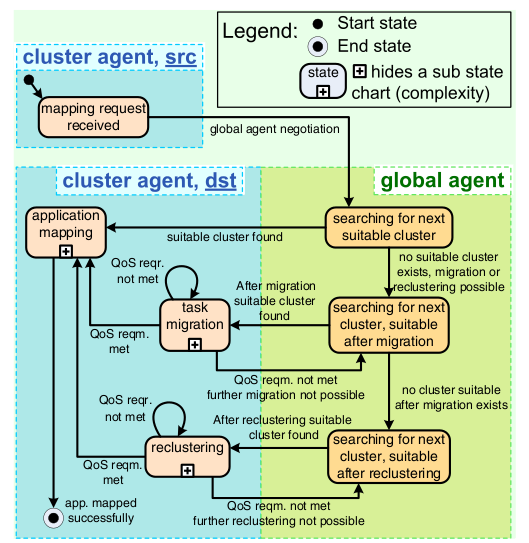
\includegraphics[width=10cm]{images/6}%
\framebox{\begin{minipage}[t]{0.2\columnwidth}%
Fig. 8\cite{4555921}%
\end{minipage}}

The run-time mapping in such a scheme is achieved by using a negotiation
policy among Cluster Agents (CAs) and Global Agents (GAs) of a certain
instance of time distributed over the whole chip. In Fig. 8 an application
mapping request is sent to the CA of the requesting cluster which
receives all mapping requests and negotiates with the GAs. There can
be multiple instances of the GAs that are synchronized over time.
The GAs have global information about all the clusters of the NoC
in order to make decisions onto which cluster the application should
be mapped to. Possible replies to this mapping request are: 

1. When a suitable cluster of the application exists then the GAs
inform the requesting source CA and the requesting source CA asks
the suitable destination CA for the actual mapping of the application. 

2. When no suitable clusters are found by the GAs then the GAs report
the next most promising cluster where it is possible to map the application
to after task migration which is negotiated between the GA and the
CA to make this cluster suitable for the mapping. The number of iterations
is a configuration parameter. 

This is targeted at reducing the problem of hotspot , by making decisions
at a lower level. The communication of agents with the global agent
is sparse and thus reduces the overhead traffic, along with the associated
congestion.


\paragraph{Incremental Mapping}

Chou et al \cite{4627545} proposed an incremental mapping scheme
that is performance aware and takes into account the possiblity of
scheduling of new jobs. They suggest a new cluster selection called
near-convex region cluster. They assume a central manager and separate
control network.

\includegraphics[width=7cm]{images/image}\includegraphics[width=8cm]{images/image}

As such, all the previous works mentioned earlier do not maximize
the system efficiency by considering the possible addition of new
applications and NoC-based communication.They claim to optimize the
communication energy consumption for all possible system configurations
(at different time instances), considering that applications can dynamically
arrive and leave the system. 


\subsubsection{Decentralized Mapping}

The idea of decentralized mapping has had only limited support in
terms of researchers working on it. As already mentioned , the field
is in a nascent stage , with no robust algorithm that can ensure order
and performance alongside the chaos that decentralized algorithm brings.
Despite the fact, there have been a handful of attempts at addressing
the problem by assuming certain restricting characteristics of the
tasks that run on the NoC. One such special case is considered in
the next chapter.
